\section{\acl{FPGA}}
\label{sec:fpga}

\acf{FPGA} merupakan sebuah perangkat keras yang mampu direkonfigurasi menggunakan sebuah bahasa \ac{HDL} \parencite{smith2024FPGA}. \ac{FPGA}, sebagai perangkat keras yang \textit{reconfigurable}, mulai marak digunakan sebagai basis perangkat keras untuk mendesain maupun mengimplementasikan akselerator perangkat keras untuk optimasi permasalahan komputasi \parencite{gerlach2023fpgaplacement}.

Secara prinsip, \ac{FPGA} terdiri atas \textit{Configurable Logic Blocks} yang dibangun diatas rangkaian \textit{Look Up Table}. Ilustrasi internal dari \ac{FPGA} dapat ditinjau pada gambar \ref{fig:ilustrasi-internal-fpga}.

\begin{figure}[h]
	\centering
	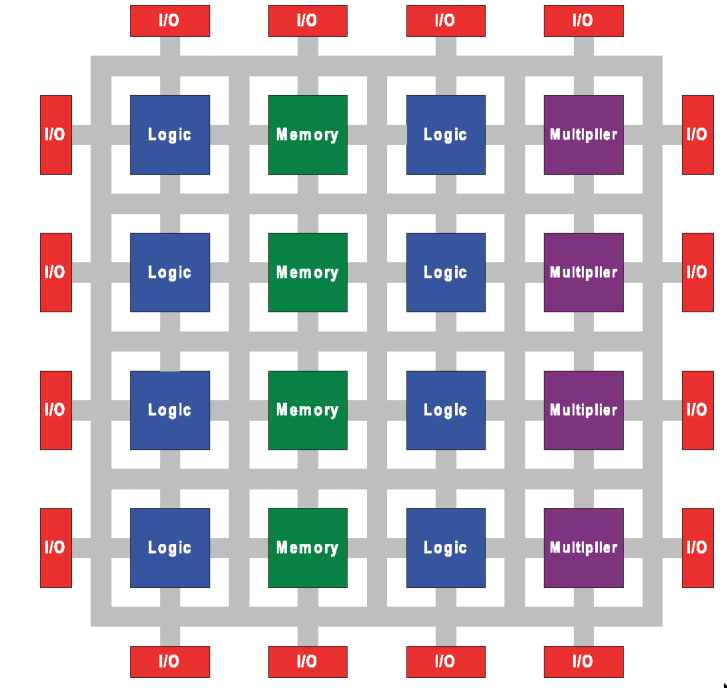
\includegraphics[width=0.6\textwidth]{chapter-2/fpga-internal.jpg}
	\caption{Ilustrasi internal \ac{FPGA} \parencite{md2015field}}
	\label{fig:ilustrasi-internal-fpga}
\end{figure}

Pada tugas akhir ini, akselerator perangkat keras yang akan diimplementasikan dan diuji pada \ac{FPGA}. Perangkat \ac{FPGA} yang digunakan adalah Nexys A7-100T yang memiliki spesifikasi sebagaimana dideskripsikan oleh tabel \ref{tab:nexys-specs}.

\begin{table}[h]
	\caption{Spesifikasi \ac{FPGA} Nexys A7-100T}
	\label{tab:nexys-specs}
	\vspace{0.25cm}
	\begin{center}
		\begin{tabular}{|c|c|}
			\hline
			Komponen Perangkat Keras        & Jumlah \tabularnewline
			\hline
			\textit{\ac{LUTs}}              & 63.400 \tabularnewline
			\textit{Flip-flops}             & 126,800 \tabularnewline
			\textit{Block \ac{RAM}}         & 4,860 Kb \tabularnewline
			\textit{DSP Slices}             & 240 \tabularnewline
			\textit{Clock Management Tiles} & 6 \tabularnewline
			\hline
		\end{tabular}
	\end{center}
\end{table}

Hasil desain akselerator, akan kemudian dilihat efisiensinya dengan mengacu kepada penggunaan jumlah penggunaan komponen perangkat keras yang tercantum pada tabel \ref{tab:nexys-specs}.
